\chapter{Classes and Objects}
\label{chap:oop}

\idx[object-oriented programming]{Object-oriented programming} is a programming paradigm that focuses on objects such as a persons, places, things, events, and concepts relevant for the problem.

Object-oriented programming has a rich language for describing objects and their relations, which can seem overwhelming at first, and they will be explained in detail in this and following chapters. Here is a brief overview: The main programming structures are called a \idx[class]{classes} and \idx[object]{objects}. It is useful to think of classes as user defined types and objects as values of such types. However, there is more to classes and objects than types and values. Objects may contain both data and code, and it is sometimes useful to draw the corresponding class definition as shown in \Cref{fig:aClass}.
\begin{figure}
  \centering
  \begin{tikzpicture} 
      \begin{class}[text width=7cm]{aClass}{0,0} 
        \attribute{// The object's values (properties)}
        \attribute{aValue : int}
        \attribute{anotherValue : float*bool}
        \operation{// The object's functions (methods)}
        \operation{aMethod:  () -> int }
        \operation{anotherMethod:  float -> float }
      \end{class}
  \end{tikzpicture}
  \caption{A class is sometimes drawn as a figure.}
  \label{fig:aClass}
\end{figure}
In this illustration, objects of type \lstinline{aClass} will each contain an int and a pair of a float and a boolean, and each object has two functions associated with them. The values stored in each object may differ, but the types are fixed by the class definition. It is common to call an object's values \idx{properties} and an object's functions \idx[method]{methods}. In short, properties and methods are collectively called \idx[member]{members}. When an object is created, memory is set aside on \idx{The Heap} to each object's property. Creating an object is commonly called \idx[instantiate]{instantiation}. The members serve as the interface to each object, and each instantiated object will have the same type of members as all objects of that class, but their content may differ.

Object-oriented programming is an extension of data types, in the sense that objects contain both data and functions in a similar manner as a module, but object-oriented programming emphasizes the semantic unity of the data and functions. Thus, objects are often \idx{models} of real-world entities, and object-oriented programming leads to a particular style of programming analysis and design called \idx[object-oriented analysis]{object-oriented analysis and design}\idxs{object-oriented design} to be discussed in \Cref{chap:oopp}. 

\section{Constructors and Members}
\label{sec:constructor}
A class is defined using the \keyword{type} keyword. Note that there are \emph{always} parentheses after the class name to distinguish it from a regular type definition. The basic syntax for a class definition is as follows:%
%
\begin{verbatimwrite}{\ebnf/simpleClass.ebnf}
type <*classIdent*> ({*<*arg*>*}) [*as <*selfIdent*>*] 
  {*let <*binding*> |* do <*statement*>*}
  {*member <*memberDef*>*}
\end{verbatimwrite}
\syntax{\ebnf/simpleClass.ebnf}{Syntax for simple class definitions.}
%
The first line is the header of the class, where the \lstinline[language=syntax]{<*classIdent*>} is the name of the class, \lstinline[language=syntax]{<*arg*>} are its optional arguments, and \lstinline[language=syntax]{<*selfIdent*>} is an optional \idx{self identifier}. The body of a class consists of the constructor and the member section. The header and the constructor section is often collectively called the \idx{constructor}, and the body of the constructor consist of optional \lstinline{let}-bindings and \lstinline{do}-statements. Note that the \lstinline{do}-statements in a class definition \emph{must} use the \lstinline{do}-keyword. The member section consisting of all the optional member definitions, where each definition use the \lstinline{member}-keyword.
%In rare instances, it is necessary to define classes that are mutably recursive, in which case the \lstinline{and}-keyword is used to combine the two definitions.\idxs{recursive classes} For example, if the definition of \lstinline{aClass} and \lstinline{bClass} depend on each other, then the combined definition should be similar to \lstinline{type aClass () = ... and bClass () = ...}.

%These define \idx{values} and \idx{functions}, which can only be accessed in the member section. They are as such private
%The \idx{primary constructor} is everything until the first member.
%Do statements must use the \lstinline{do}-keyword.

The header and constructor section is commonly called the \idx{constructor}, and the constructor is executed at instantiation. In contrast to many other languages, the constructor is always stated as the initial code of a class definition.
% It is called the \idx{primary constructor}, its arguments are specified in the header, and the primary constructor's body is the \keyword{let} and \keyword{do}-bindings following the header.
The values and variables in the constructor are called \idx[field]{fields}, while functions are just called \idx{functions}.

Members are declared using the \idx[member@\keyword{member}]{\keyword{member}}-keyword, which defines values and functions that are accessible from outside the class using the \lexeme{.}-notation. In this manner, the members define the \idx{interface} between the internal bindings in the constructor and an application program. Member values are called \idx{properties}, and
% Note that the concept of properties as member values is different from the concept of functions and \lstinline{let}-binding properties, which is specified with the \lstinline{[<>]} notation. For this reason, this author prefers the name member property in F\#.
member functions are called \idx[method]{methods}. Note that members are immutable.
% In the example in \Cref{class}, line~\ref{classMemberValue} and~\ref{classMemberFunction} define a property and a method. Properties and methods 'belong to' or 'resides in' objects.
The body of a member has access to the arguments, the constructor's bindings, and to all class members, regardless of the member's lexicographical order. 
%One way to think about objects is that properties are the object's \idx{state} and methods are \idx{messages} sent between the object and its application program.
In contrast, members are not available in the constructor unless the self identifier has been declared in the header using the keyword \idx{\keyword{as}}, e.g., \lstinline{type classMutable(name : string) as this = ...}.

Consider the example in \Cref{fig:instantiation}.
\begin{figure}
  \centering
  \begin{tikzpicture} 
      \begin{class}[text width=4cm]{car}{0,0} 
        \attribute{// A car has a color}
        \attribute{color : string}
      \end{class}
      \begin{object}[text width=4cm]{sportsCar}{-5,-2.5}
        \instanceOf{car}
        \attribute{color = ``red''}
      \end{object}
      \begin{object}[text width=4cm]{stationWagon}{0,-2.5}
        \instanceOf{car}
        \attribute{color = ``green''}
      \end{object}
      \begin{object}[text width=4cm]{miniBus}{5,-2.5}
        \instanceOf{car}
        \attribute{color = ``blue''}
      \end{object}
    \end{tikzpicture}
  \caption{A class \lstinline{car} is instantiated trice and bound to the names \lstinline{sportsCar}, \lstinline{stationWagon}, and \lstinline{miniBus}, and each object's properties are set to different values.}
  \label{fig:instantiation}
\end{figure}
Here we have defined a class \lstinline{car}, instantiated three objects, and bound them to the names \lstinline{sportsCar}, \lstinline{stationWagon}, and \lstinline{miniBus}. Each object has been given different values for the \lstinline{color} property. In F\# this could look like the code in \Cref{car}.
%
\fs{car}{Defining a class car, and making three instances of it. See also \Cref{fig:instantiation}.}%
%
In the example, the class \lstinline{car} is defined in lines~\ref{carHeader}--\ref{carMemberEnd}. Its header includes one string argument, \lstinline{aColor}. The body of the constructor is empty, and the member section consists of lines~\ref{carMemberStart}--\ref{carMemberEnd}. The class defines one property \lstinline{color : string}. Note that when referring to a member inside an object, then we must use a \idx{self identifier}. Here we use \lstinline{this} as the self identifier, and as the example shows, we need not declare it in the class' header. A self identifier refers to the memory set aside to the particular instance of an object. It is common among other programming languages to use \lstinline{this} as self identifier. F\# is very flexible regarding what name can be used for the self-identifier, and the member section could as well have been \lstinline{self.value}, \lstinline{__.value}, or anything else, and it need not be the same in every member definition. Nevertheless, \advice{consistency in the name used as self-identifier is strongly encouraged, preferably using a name that reflects the nature of the reference, such as \lstinline{this} or \lstinline{me}.} The objects are instantiated in lines~\ref{carObject1}--\ref{clarObject3}, and the value of their properties are accessed in line~\ref{carObjectUse}. In many languages, objects are instantiated using the \idx[new@\lstinline{new}]{\keyword{new}} keyword, but in F\# this is optional. I.e., \lstinline{let sportsCar = car ("red")} is identical to \lstinline{let sportsCar = new car ("red")}. Note that both the self identifier and member access uses the \lexeme{.} notation.

A more advanced implementation of a \lstinline{car} class might include notions of a fuel gauge, fuel economy, and the ability to update the fuel gauge as the car is driven. An example of an implementation of this is given In \Cref{class}.
%
\fs{class}{Extending \Cref{car} with fields and methods.}%
%
Here in line~\ref{classHeader}, the constructor has 2 arguments: the fuel economy parameter and the initial amount of fuel in the tank. Thus, we are able to create 2 different cars with different fuel economy, as shown in lines~\ref{classObject}--\ref{classObject2}. The amount of fuel left en each car object is stored in the mutable field \lstinline{fuelLeft}. This is an example of a state of an object: It can be accessed outside the object by the \lstinline{fuel} property, and it can be updated by the \lstinline{drive} method. 

Field names and functions defined in the constructor do not use the self identifier and cannot be accessed outside and object using the \lexeme{.} notation. However, they are available in both the constructor and the member section following the regular scope rules. Fields are a common way to hide implementation details, and they are \idx{private} to the object or class in contrast to members that are \idx{public}.

\begin{comment}
Tuple arguments to class constructors causes a special problem in F\#, since both constructions uses parentheses. the call to the constructor looks identical. This is demonstrated in \Cref{classTuple}.
%
\fsCode{classTuple}{classTuple}{Beware: Creating objects from classes with several arguments and tuples have the same syntax.}{}
%
Whether the full list of arguments should be transported from the caller to the object as a tuple or not is a matter of taste that mainly influences the header of the class. The same cannot be said about how the elements of the vector are stored inside the object and made accessible outside the object. In \Cref{classTuple}, the difference between storing the vector's elements in individual members \lstinline{member this.x = x} and \lstinline{member this.y = y} or as a tuple \lstinline{member this.cartesian = (x, y)}, is that in order to access the first element in a vector \lstinline{v}, an application program in the first case must write \lstinline{v.x}, while in the second case the application program must first retrieve the tuple and then extract the first element, e.g., as \lstinline{fst v.cartesian}. Which is to be preferred depends very much on the application: Is it the individual elements or the complete tuple of elements that is to have focus, when using the objects. Said differently, which choice will make the easiest to read application program with the lowest risk of programming errors. Hence, when designing classes, \advice{consider carefully how application programs will use the class and aim for simplicity and versatility while minimizing the risk of error in the application program.}
\end{comment}

\section{Accessors}
Methods are most often used as an interface between the fields of an object and the application program. Consider the example in \Cref{classAccessor}.
%
\fs{classAccessor}{Accessor methods interface with internal bindings.}
% 
In the example, the data contained in objects of type \lstinline{aClass} is stored in the mutable field \lstinline{v}. Since only members can be accessed from an application, it is not possible to retrieve or change the data of these object of class \lstinline{aClass} directly. We could have programmed \lstinline{v} as a member instead, i.e., \lstinline{member this.v = 1}, however, often we are in a situation, where there is a range of possible choices of data representation, details of which we do wish to share with an application program. E.g., implementation details of arrays are not important for our ability to use them in applications. What matters is that the members that work on the array elements are well defined and efficient. Thus, the example demonstrates how we can build two simple methods \lstinline{setValue} and \lstinline{getValue} to set and get the data stored \lstinline{v}. By making a distinction between the internal representation and how members give access to the data, we retain the possibility to change the internal representation without having to reprogram all the application programs. Analogously, we can change the engine in a car from one type to another without having to change the car's interaction with the driver and the road: steering wheel, pedals, wheels etc.

Such functions are called \idx{accessors}.  Internal states with setters and getters are a typical construction, since they allow for complicated computations when states are read to and written from, and gives the designer of the class the freedom to change the internal representation while keeping the interface the same. Accessors are so common that F\# includes a special syntax for them: Classes can be made to act like variables using \keyword{member}\dots\keyword{with}\dots\keyword{and} keywords and the special function bindings \keyword{get()} and \keyword{set()}, as demonstrated in \Cref{classGetSet}.
%
\fs{classGetSet}{Members can act as variables with the built-in get and set functions.}
% 
The expression defining \lstinline{get: () -> 'a} and \lstinline{set: 'a -> ()}, where \lstinline{'a} is any type, can be any usual expression. The application calls the \lstinline{get} and \lstinline{set} as if the property were a mutable value. If \lstinline{set} is omitted, then the property acts as a value rather than a variable, and values cannot be assigned to it in the application program.

Setters and getters are so common that F\# has a short-hand for this using \keyword{member val value = 0 with get, set}, which creates the internal mutable value \lstinline{value}, but this is discouraged in this text.

Defining an \idx{\lstinline{Item}} property with extended \lstinline{get} and \lstinline{set} makes objects act as indexed variables, as demonstrated in \Cref{classGetSetIndexed}.
%
\fs{classGetSetIndexed}{Properties can act as indexed variables with the built-in get and set functions.}
% 
Higher dimensional indexed properties are defined by adding more indexing arguments to the definition of \lstinline{get} and \lstinline{set}, such as demonstrated in \Cref{classGetSetHigherIndexed}.
%
\fs{classGetSetHigherIndexed}{Getters and setters for higher dimensional index variables.}
% 

% ********  Setters and getters are so common that F\# has a short-hand for this using a combination of \keyword{member}, \keyword{val}, \keyword{}, \keyword{get}, and \keyword{set} as shown \Cref{classSetGetShort}.\jon{I'm considering to remove explicit examples using \lstinline{member val} to reduce language subset.}
% %
% \fs[linebackgroundcolor={%
% \highlight{\getrefnumber{classSetGetShortMemberValGetSet}}%
% }]{classSetGetShort}{A short-hand for setters and getters. Compare with \Cref{classSetGet}.}
% %
% In the example line~\ref{classSetGetShortMemberValGetSet}, the binding sets the default values, and omitting any of the \keyword{get}- and \keyword{set}-keywords removes the read and write property of the variable from the application program.\jon{possibly add something about \keyword{private}.}

\begin{comment}
Combinations of non-static member definitions are shown in \Cref{classMemberDefinition}.
%
\fsCode{classMemberDefinition}{classMemberDefinition}{A large variation of class member definitions. This program intentionally does not compile, but demonstrates variation that will, and problematic lines are indicated by the in-code comments.}{}
%
The \lstinline{val}-keyword in this context has not been discussed previously.\jon{maybe mention ``Explicit Field'', \url{https://docs.microsoft.com/en-us/dotnet/fsharp/language-reference/members/explicit-fields-the-val-keyword}.} \lstinline{staticMemberV} and \lstinline{staticMemberValV} have the same interface. The \lstinline{[<DefaultValue>] val mutable valMutableV : int} has not been discussed and is discouraged, but gives a mutable property that is initialized to the type's default value, e.g., \lstinline{Unchecked.defaultof<int>} in this case. \idx{\lstinline{[<DefaultValue>]}} is called an \idx{attribute}, but will not be discussed further.\jon{Should attributes be included \url{https://docs.microsoft.com/en-us/dotnet/fsharp/language-reference/attributes}?} Defining mutable properties is illegal, but allowed using explicit get and set functions. The definitions for \lstinline{valMutableV}, \lstinline{memberValGetSetV} and \lstinline{memberThisGetSetV} gives the same interface to a mutable variable, but with slight variation in how their initial value is set, and how get and set actions can be programmed. In general, \advice{minimize the use of constructions using the \keyword{val}-keyword in class definitions for brevity.}  All the above holds for static definitions except \lstinline{[<DefaultValue>] static val mutable staticValMutableV : int} is illegal.

\end{comment}
\section{Objects are Reference Types}
Objects are reference type values, implying that copying objects copies their references, not their values, and their content is stored on \idx{The Heap}, see \Cref{sec:referenceCells}. Consider the example in \Cref{classReference}.
%
\fs{classReference}{Objects assignment can cause aliasing.}
%
Thus, the binding to \lstinline{b} in line~\ref{classReferenceAlias} is an alias to \lstinline{a}, not a copy, and changing object \lstinline{a} also changes \lstinline{b}! This is a common cause of error, and you should \advice{think of objects as arrays.} For this reason, it is often seen that classes implement a copy function returning a new object with copied values, e.g., \Cref{classCopy}.
%
\fs{classCopy}{A copy method is often needed. Compare with \Cref{classReference}.}
%
In the example, we see that since \lstinline{b} now is a copy, we do not change it by changing \lstinline{a}. This is called a \idx{copy constructor}.

\section{Static Classes}
Classes can act as modules and hold data which is identical for all objects of its type. These are defined using the \idx[static@\keyword{static}]{\keyword{static}}-keyword. And since they do not belong to a single object, but are shared between all objects, they are defined without the self-identifier and accessed using the class name, and they cannot refer to the arguments of the constructor. For example, consider a class whose objects each hold a unique identification number (id): When an object is instantiated, the object must be given the next available identification number. The next available id could be given as an argument to the constructor, however, this delegates the task of maintaining the uniqueness of ids to the application program. It is better to use a static field and delegate the administration of ids completely to the constructors, as demonstrated in \Cref{classStatic}.
%
\fs{classStatic}{Static fields and members are identical to all objects of the type.}
%
Notice in line~\ref{classStaticStaticField} that a static field \lstinline{nextAvailableID} is created for the value to be shared by all objects. The initialization of its value is only performed once, at the beginning of program execution. However, every time an object is instantiated, the value of \lstinline{nextAvailableID} is copied to the object's field \lstinline{studentID} in line~\ref{classStaticNonStaticField}, and \lstinline{nextAvailableID} is updated. The static field can be accessed with a static accessor, as demonstrated in line~\ref{classStaticStaticMemeber}. Notice how this definition does not include a self-identifier, and that the member is accessible from the application in line~\ref{classStaticStaticAccess} using the class' name, in both cases since it is not a member of any particular object.

\section{Recursive Members and Classes}
The members of a class are inherently recursive: static and non-static methods may recurse using the self identifier and other members regardless of their lexicographical scope. This is demonstrated in \Cref{classRecursion}.
%
\fs{classRecursion}{Members can recurse without the \lstinline{rec} keyword and refer to other members regardless of their lexicographical scope.}
%
For mutually recursive classes, the keyword \idx{\keyword{and}} must be used, as shown in \Cref{classAssymetry}.
%
\fs{classAssymetry}{Mutually recursive classes are defined using the \keyword{and} keyword.}
%
Here \lstinline{anInt} and \lstinline{aFloat} hold an integer and a floating point value respectively, and they both implement an addition of \lstinline{anInt} an \lstinline{aFloat} that returns and \lstinline{aFloat}. Thus, they are mutually dependent and must be defined in the same \keyword{type} definition using \keyword{and}.

\section{Function and Operator Overloading}
It is often convenient to define different methods that have the same name, but with functionalities that depend on the number and type of arguments given. This is called \idx{overloading}, and F\# supports method overloading. An example is shown in \Cref{classOverload}.
%
\fs{classOverload}{Overloading methods \lstinline{set : int -> ()} and \lstinline{set : int * int -> ()} is permitted, since they differ in argument number or type.}
% 
In the example we define an object which can produce greetings strings of the form \lstinline[language=syntax]{<*greeting*> <*name*>}, using the \lstinline{str} member. It has a default greeting ``Hi'' and name ``Programmer'', but the name can be changed by calling the \lstinline{setName} accessor with one argument, and both greeting and name can be changed by calling the overloaded \lstinline{setName} with two arguments. Overloading in class definition is allowed as long as the arguments differ in number or type.

In \Cref{classAssymetry}, the notation for addition is less than elegant. For such situations, F\# supports \idx{operator overloading}. All usual operators may be overloaded (see \Cref{sec:operators}), and in contrast to regular operator overloading, the compiler uses type inference to decide which function is to be called. All operators have a functional equivalence, and to overload the binary \lexeme{+} and unary \lexeme{-} operators, we overload their functional equivalence \lstinline{(+)} and \lstinline{(~-)} as static members. This is demonstrated in \Cref{classOverloadOperator}.
%
\fs{classOverloadOperator}{Operators can be overloaded using their functional equivalents.}
% 
Thus, writing \lstinline{v + w} is equivalent to writing \lstinline{anInt.(+) (v, w)}. Presently, the former is to be preferred, but at times, e.g., when using functions as arguments, it is useful to be able to refer to an operator by its function-equivalent. Note that the functional equivalence of the multiplication operator \lstinline{(*)} shares a  prefix with the begin block comment lexeme \lexeme{(*}, which is why the multiplication function is written as \lstinline{( * )}. Note also that unitary operators have a special notation using the \lexeme{\~}-lexeme, as illustrated in the above example for unitary minus. With the unitary minus, we are able to subtract objects of \lstinline{anInt} by first negating the right-hand operand and then adding the result to the left-hand operand. In contrast, the binary minus would have been defined as \lstinline{static member (-) (v : anInt, w : aFloat) = anInt ((float v.value) - w.value)}.

In \Cref{classOverloadOperator}, notice how the second \lstinline{(+)} operator overloads the first by calling the first with the proper order of arguments. This is a general principle: \advice{avoid duplication of code, reuse of existing code is almost always preferred.} Here it is to be preferred for two reasons. Firstly, if we discover a mistake in the multiplication code, then we need only correct it once, which implies that both multiplication methods are corrected once and reduces the chance of introducing new mistakes by attempting to correct old ones. Secondly, if we later decide to change the internal representation, then we only need to update one version of the multiplication function, hence we reduce programming time and risk of errors as well.

Beware that operator overloading outside class definitions overwrites \emph{all} definitions of the operator. E.g., overloading \lstinline{(+) (v, w)} outside a class will influence integer, real, string, etc. Thus, \advice{operator overloading should only be done inside class definitions.}
%\jon{Something about which operators can be overloaded \url{https://docs.microsoft.com/en-us/dotnet/fsharp/language-reference/operator-overloading}.}

%Overloading is a programming structure that does not work well in functional-first programming languages such as F\# since types are not easily inferred. Therefore, overloading has restricted usage. E.g., even in the above case, if the application program attempts to define the following function \lstinline{let f = anInt.(+)}, the functional equivalent of the \lexeme{+} operator, then the compiler will not be able to identify, which of the two candidate functions are to be bound to \lstinline{f}, and will throw an error. Although irrelevant until \lstinline{f} is applied to arguments, an effective type inference system has yet to be implemented.

\section{Additional Constructors}
Like methods, constructors can also be overloaded by using the \idx[new@\lstinline{new}]{\lstinline{new}} keyword. E.g., the example in \Cref{classOverload} may be modified, such that the name and possibly greeting is set at object instantiation rather than by using the accessor. This is illustrated in \Cref{classExtraConstructor}.
%
\fs[linebackgroundcolor={%
\highlightRange{\getrefnumber{classExtraConstructorStart}}{\getrefnumber{classExtraConstructorEnd}}%
\highlight{\getrefnumber{classExtraConstructorAddApp}}%
\highlight{\getrefnumber{classExtraConstructorPrimApp}}%
}]{classExtraConstructor}{Extra constructors can be added, using \keyword{new}.}
%
The top constructor that does not use the \lstinline{new}-keyword is called the \idx{primary constructor}. The body of the additional constructor must call the primary constructor, and the body cannot extend the primary constructor's fields and functions. It is useful to \advice{think of the primary constructor as a superset of arguments and the additional ones as subsets or specializations.} As regular scope rules dictate, the additional constructor has access to the primary constructor's bindings. However, in order to access the object's members, the self identifier has to be explicitly declared, using the \keyword{as}-keyword in the header. E.g., writing \lstinline{new(x : float, y : float) as alsoThis = ...}. However beware. Even though the body of the additional constructor now may access the property \lstinline{alsoThis.x}, this value has first been created once the primary constructor has been called. E.g., calling the primary constructor in the additional constructor as \lstinline{new(x : float, y : float) as alsoThis = classExtraConstructor(fst alsoThis.x, y, defaultSeparator)} will cause an exception at runtime. Code may be executed in additional constructors: Before the call to the primary constructor, \keyword{let} and \keyword{do} statements are allowed. If code is to be executed after the primary constructor has been called, then it must be preceded by the \keyword{then} keyword, as shown in \Cref{classDoThen}.
%
\fs[linebackgroundcolor={%
\highlightRange{\getrefnumber{classDoThenDoStart}}{\getrefnumber{classDoThenDoEnd}}%
\highlightRange{\getrefnumber{classDoThenDoAddStart}}{\getrefnumber{classDoThenDoAddEnd}}%
\highlightRange{\getrefnumber{classDoThenThenStart}}{\getrefnumber{classDoThenThenEnd}}%
}]{classDoThen}{The optional \keyword{do}- and \keyword{then}-keywords allow for computations before and after the primary constructor is called.}
%
The \keyword{do}-keyword is often understood to be implied by F\#, e.g., in front of all \lstinline{printf}-statements, but in the above examples they are required where used. This may change in future releases of F\#. F\# allows for many additional constructors, but they must be distinguishable by type.

\section{Programming Intermezzo: Two Dimensional Vectors}
Consider the following problem.
\begin{problem}
  A Euclidean vector is a geometric object that has a direction, a length, and two operations: vector addition and scalar multiplication, see \Cref{fig:vectorAddition}. Define a class for a vector in two dimensions.
\end{problem}
\begin{figure}
  \centering
  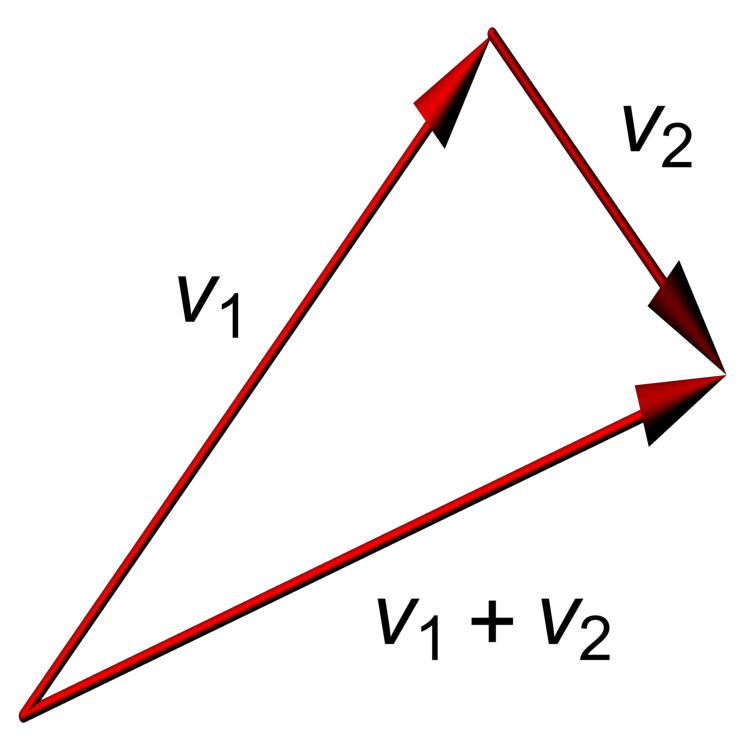
\includegraphics[width=0.45\textwidth]{vectorAddition}
  \caption{Illustration of vector addition in two dimensions.}
  \label{fig:vectorAddition}
\end{figure}
An essential part in designing a solution for the above problem is to decide which representation to use internally for vectors. The Cartesian representation of a vector is as a tuple of real values $(x,y)$, where $x$ and $y$ are real values, and where we can imagine that the tail of the vector is in the origin, and its tip is at the coordinate $(x,y)$. For vectors on Cartesian form,
\begin{align}
  \vec v = (x,y),
\end{align}
the basic operations are defined as
\begin{align}
  \vec v_1 + \vec v_2 &= (x_1+x_2, y_1+y_2),
  \\a\vec v &= (a x,a x),
  \\\text{dir}(\vec v) &= \tan\frac{y}{x},\, x\neq 0,
  \\\text{len}(\vec v) &= \sqrt{x^2+y^2},
\end{align}
where $x_i$ and $y_i$ are the elements of vector $\vec v_i$, $a$ is a scalar, and $\text{dir}$ and $\text{len}$ are the direction and length functions, respectively. The polar representation of vectors is also a tuple of real values $(\theta, l)$, where $\theta$ is the vector's angle from the $x$-axis and $l$ is the vector's length. This representation is closely tied to the definition of a vector, and has the constraint that $0 \leq \theta < 2\pi$ and $0 \leq l$. This representation reminds us that vectors do not have a position. For vectors on polar form,
\begin{align}
  \vec v &= (\theta,l),
\end{align}
their basic operations are defined as
\begin{align}
  x(\theta,l) &= l\cos(\theta),
  \\y(\theta,l) &= l\sin(\theta),
  \\\vec v_1 + \vec v_2 &= (x(\theta_1,l_1)+x(\theta_2,l_2), y(\theta_1,l_1)+y(\theta_2,l_2))
  \\a\vec v &= (\theta,a l),
\end{align}
where $\theta_i$ and $l_i$ are the elements of vector $\vec v_i$, $a$ is a scalar, and $\text{x}$ and $\text{y}$ are the Cartesian coordinate functions.

So far in our analysis, we have realized that:
\begin{itemize}
\item both the Cartesian and polar representations use a pair of reals to represent the vector, 
\item both require functions to calculate the elements of the other representation, 
\item the polar representation is invalid for negative lengths, and
\item the addition operator under the polar representation is also more complicated and essentially requires access to the Cartesian representation.
\end{itemize}
 

The first step in shaping our solution is to decide on file structure: For conceptual separation, we choose to use a library and an application file. F\# wants files to define namespaces or modules, so we choose the library to be a \lstinline{Geometry} module, which implements the vector class to be called \lstinline{vector}. Furthermore, when creating vector objects we would like to give the application program the ability to choose either Cartesian or polar form. This is can be done using \idx{discriminated unions}. Discriminated unions allow us to tag values of possibly identical form, but they also lead to longer programs. Thus, we will also provide an additional constructor on implicit Cartesian form, since this is the most common representation of vectors.

A key point when defining libraries is to consider their interface with the application program. Hence, our second step is to write an application using the yet to be written library in order to get a feel for how such an interface could be. This is demonstrated in the application program \Cref{vectorAppCode}.
%
\fsCode{vectorApp}{vectorAppCode}{An application using the library in \Cref{vector}.}{}
%
The application of the vector class seems natural, makes use of the optional discriminated unions, uses the infix operators \lexeme{+} and \lexeme{*} in a manner close to standard arithmetic, and interacts smoothly with the \lstinline{printf} family. Thus, we have further sketched requirements to the library with the emphasis on application.

After a couple of trials, our library implementation has ended up as shown in \Cref{vector}.
%
\fsImplementation{vector}{vector}{A library serving the application in \Cref{vectorApp}.}{}
%
Realizations achieved during writing this code are: Firstly, in order to implement a vector class using discriminated unions, we had to introduce a constructor with helper variables \lstinline{_x}, \lstinline{_y}, etc. The consequence is that the Cartesian and polar representation is evaluated once and only once every time an object is created. Unfortunately, discriminated unions do not implement guards on subsets, so we still have to cast an exception when the application attempts to create an object with a negative length. Secondly, for the \lstinline{ToString} override we have implemented static members for typesetting vectors, since it seems more appropriate that all vectors should be typeset identically. Changing typesetting thus respects dynamic scope.

The output of our combined library and application is shown in \Cref{vectorApp}.
%
\fsOutput{vectorApp}{Compiling and running the code from \Cref{vector} and~\ref{vectorAppCode}.}
%
The output is as expected, and for the vector class, our solution seems to be a good compromise between versatility and syntactical bloating.

%%% Local Variables:
%%% TeX-master: "fsharpNotes"
%%% End:

